\documentclass[10pt]{article}
\usepackage[utf8]{inputenc}
\usepackage[T1]{fontenc}
\usepackage{lmodern}
\usepackage[italian]{babel}
\usepackage{multicol}
\usepackage[a4paper, total={18cm, 25cm}]{geometry}
\usepackage{array}
\usepackage{graphicx}
\graphicspath{ {./img/} }

\begin{document}
\title{Programmazione d'Interfacce}
\author{Federico Matteoni}
\date{ }
\renewcommand*\contentsname{Indice}

\maketitle
\tableofcontents
\pagebreak
\section{Introduzione}
Appunti del corso di \textbf{Programmazione d'Interfacce} presi a lezione da \textbf{Federico Matteoni}.\\More like \textit{design d'interfacce}.\\\\
Prof.: \textbf{Daniele Mazzei}, mazzei@di.unipi.it\\
\begin{list}{-}{Riferimenti web:}
\item \emph{?}
\end{list}
Esame: compitini/scritto. \textbf{Facoltativo}: orale discorsivo dove si discute un software noto.\\Possibile proporre un software personale da presentare all'esame orale, spiegando come si è applicati i rudimenti del corso sul software presentato.\\\\
\begin{list}{-}{Materiale didattico:}
\item \textbf{Google Classroom}, slide presentate a lezione e altro materiale didattico\\Codice \textbf{c14kiy} con le credenziali d'ateneo.\\La suite Google è attivabile a \emph{start.unipi.it/gsuite}\\\textit{Non è autorizzata la divulgazione}
\item La Caffettiera del Masochista, Donald A. Norman\\Eng: The Design of Everyday Things
\item Designing the User Interface, Ben Shneiderman
\item \emph{www.usability.gov}
\item \emph{interaction-design.org}
\end{list}
Ricevimento: Mercoledì 14.30-16, Stanza 366\\

\section{Il Corso}
\textbf{Interface Development in 2020} diventa \textbf{Interface Design in 2020}
\paragraph{Diviso in due parti}
\begin{list}{-}{}
\item \textbf{UX e UI} con introduzione, UI vs UX, HCI, paradigmi, gamification...
\item \textbf{Strumenti per lo sviluppo dell'interfaccia utente} presentati da vari ospiti: Unity, Zerynth, Ubidots, Angular, Amazon Lex, ...
\end{list}

\textbf{Interfaccia} è qualsiasi metodo utilizzato da una persona per \textbf{interagire} con un dispositivo.

\section{Design}
\paragraph{Cos'è il design} Il design è la \textbf{pianificazione o la specifica per la costruzione di un oggetto o sistema} o per l'implementazione di un'attività o processo. Diventa l'esatto opposto della decomposizione del problema in sottopassaggi, cioè del pensiero computazionale. Il design parte dalla base del problema e \textbf{identifica soluzioni per la causa del problema}. Si può avere anche il design di una strategia di implementazione.\\
\quotedblbase \textbf{Bisognerebbe progettare le applicazioni come se fossero persone che ci piacerebbe frequentare}\textquotedblright. Ad esempio Netflix, o il frigorifero.

\subsection{XX Designer}
Discernere tra Graphic Design, User Experience Design (UX Design) e User Interface Design (UI Design).
\paragraph{UX}: come l'utente si sente per interagire e cosa vuole fare. Aspetto più psicologico, guida la UI design in base a statistica fatta su gruppi di utenti. Manda "\textit{l'output}" a chi fa UI e al marketing.\\
\paragraph{UI}: come l'utente interagisce col prodotto (shortcut, sottomenu...)\\
\subsubsection{UX Designer}
Si deve porre il problema di quali approcci usare per risolvere problemi evidenziati da analisi di mercato.\\
\textbf{Chi paga non è detto che sia chi usa il servizio}. Ad esempio Netflix viene pagato da una persona, ma lo stesso account viene usato anche da altre persone (anzi, in particolare \textbf{il 90\% del tempo} chi usa l'account non è chi paga).\\
Uno dei metodi usati per fare UX è quello della \textbf{definizione delle \textbf{personas}} (cioè un archetipo di utente). Una persona può assumere diverse personas.
\paragraph{User Experience} Con User Experience si parla del prodotto e di come si comporta nel mondo reale, che è fatto di \textit{personas}.
\textbf{Non si può progettare \textit{una user experience}, si può progettare \textit{per la user experience}}. La user experience è ciò che fa l'utente, e lo sviluppatore non ha controllo su ciò. L'utente si approccia al software come gli pare.
\subsubsection{UI Designer}
Dalla UX si crea lo \textbf{sketch} dell'interfaccia. Non viene prodotto subito il wireframe ma bisogna partire da altro, ad esempio dai \textbf{casi di studio}. Esistono più casi di studio per ogni personas (casalinga voghera che fa bonifico, casalinga voghera che cambia password, ecc.). Ogni caso di studio è \textbf{specifico per personas}, poiché personas diverse hanno capacità diverse (non conoscere alcuni concetti, non saper fare determinate operazioni...).\\
L'\textbf{UI design è un procedimento diverso dal front-end developing}, quindi possono essere persone separate. Il designer progetta le guideline che istruiscono il developer.\\
Si può dire che la UI design è sottoarea di UX design.\\

\subsection{Front-End Developer}
Esegue il design della UI convertendolo in funzionalità del prodotto.\\

\section{Interfacce Utente}
\paragraph{L'interfaccia utente (UI)} L'UI di un sistema è \textbf{lo spazio dove avviene l'interazione uomo-macchina}: lo schermo, le casse, il mouse e quant'altro.\\
L'obiettivo dell'interfaccia è far si che \textbf{l'utente possa controllare la macchina}, e \textbf{non il contrario}. L'interfaccia può però influenzare il comportamento dell'utente, ad esempio se voglio guidare l'utente in un particolare modo l'interfaccia deve dare un feedback tale da guidare l'utente.\\
L'altro obiettivo dell'interfaccia è \textbf{rendere fruibile \textit{in maniera piacevole} le funzionalità che una macchina eroga} verso l'utente. Il termine \textbf{user-friendly} non può essere omesso: tra un'app facile e piacevole da usare e una solo facile da usare, l'utente medio preferirà sempre la prima.\\
L'interfaccia è strutturata a layer. lo HID (Human Interface Device) è la periferica con cui l'umano interagisce col sistema. Questo server per usare più HID per interagire con diverse applicazioni.\\
HMI (Human Machine Interface) è più astratta rispetto a HCI (Human Computer Interface), quindi in HMI è più teorica la cosa.
\paragraph{Diversi tipi di interfacce} Abbiamo 5 sensi, quindi diverse \textbf{categorie d'interfaccia}: le più comuni sono \textbf{grafiche} e \textbf{tattili} (\textbf{GUI}, Graphical User Interface). Se si aggiunge anche il suono diventano \textbf{MUI} (Multimedia User Interface). Il concetto di GUI è stato coniato in un tempo in cui l'audio era raro. Adesso \textbf{praticamente tutte le interfacce sono MUI}.\\
Esempio di MUI riprogettata in GUI: Facebook. I video partivano in automatico con l'audio attivo, mentre ora sono mutati. Poi sono stati aggiunti i sottotitoli automatici: questo è un esempio di tecnica ideata per le utentze disabili e riusata per poter far fruire il prodotto a quelle personas che in quel momento non possono usufruire dell'audio. \textit{Meglio un sottotitolo sbagliato che niente}.
\paragraph{Categorizzare interfacce} Le CUI (Composite User Interfaces) sono le UI che interagiscono con due o più sensi.
\begin{list}{}{Esistono tre diverse macrocategorie di CUI:}
\item \textbf{Standard}, che utilizzano dispositivi standard come tastiere, mouse e monitor
\item \textbf{Virtuale}, che \textbf{bloccano il mondo reale e creano un mondo virtuale} e tipicamente utilizzano dei caschi VR
\item \textbf{Aumentata}, che \textbf{non blocca il mondo reale e eroga contenuti non completamente digitali}, ma che prendono dalla realtà esterna che circonda l'utente
\end{list}
Le CUI possono anche essere \textbf{classficiate per il numero di sensi} con cui esse interagiscono. Per esempio, lo \textit{Smell-O-Vision} è una CUI standard 3S (3 sensi) con un display, suono e odori. Se si aggiungesse la vibrazione della poltrona, diventerebbe 4S poiché si aggiunge il tatto.\\
Si parla di \textbf{Qualia Interfaces} quando si stimolano tutti i sensi.
\paragraph{Mancata evoluzione} Le UI \textbf{sono le stesse di 10 anni fa}. Bisogna mettere in discussione i paradigmi attuali. L'industria ha convertito l'ambiente fisico della scrivania in ambiente digitale, prendendo ispirazione dall'abitudine dell'utente per rendere più semplice il passaggio. Ora l'utente è abituato, la realtà da cui si prende spunto non esiste più. Bisogna cambiare.

\section{Good and Bad Design}
\textbf{Il buon design non esiste}, poiché si fa design \textit{per} la user experience \textbf{di una determinata personas}.
\begin{list}{}{Le due caratteristiche più importanti su cui misurare il buon design sono:}
\item \textbf{Discoverability}: è la \textbf{capacità innata di un sistema di veicolare i possibili usi e dire come si usa}. Non è detto che una volta che si è capito cosa si può fare si riesca a farlo.\\
Per avere buona discoverability si usa tipicamente la visibilità: un rubinetto con i pomelli bene in vista incrementa la discoverability. Nel software, \textbf{questo lavoro lo fanno i pulsanti}.
\item \textbf{Understanding}: è la \textbf{capacità di comprendere i possibili usi}. Ad esempio: il fornello, è in cucina quindi so che si usa per scaldare ecc., il problema maggiore però è il mapping pomello $\rightarrow$ fornello. Si può risolvere con l'icona del fornello corrispondente, ma non risolve effettivamente il problema. Una soluzione efficacie è disporre fornelli e pomelli in modo che sia evidente la correlazione fra essi.\\
\textbf{Non sottovalutare il costo mentale dell'utente}.
\end{list}
\begin{center}
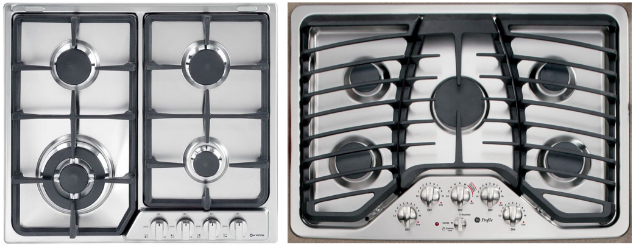
\includegraphics[scale=0.5]{fornelli.png}
\end{center}

\subsubsection{Design of Useful Things}
\paragraph{Il paradosso di TripAdvisor} \quotedblbase \emph{Quando la gente mangia bene, non recensisce. Quando mangia male, recensisce}\textquotedblright.
\paragraph{Sensazioni} Quando le cose vanno bene, si dimenticano subito. Questo perché, in qualche modo, l'uomo pensa che \textbf{le cose vadano bene per definizione}. Quando qualcosa va storto, invece, \textbf{l'amigdala crea un ricordo con un peso molto maggiore}.\\
Il design deve quindi preoccuparsi di come funzionano le cose, come vengono controllate e della natura delle interazioni. Quando la progettazione è fatta bene, crea prodotti piacevoli e brillanti. Quando è fatta male, i prodotti sono inutilizzabili e ciò porta a notevole frustrazione e irritazione.\\
\textbf{Marcatore somatico}: ricordo le esperienze in base alle sensazioni che provavo durante esse. \textbf{Più forte è la sensazione più si cementifica il ricordo}. Ad esempio se faccio un incidente ad una curva, la ricorderò bene per molto tempo. La strada che faccio per andare in vacanza non la ricordo più già al ritorno.\\
\textbf{Con il software si applica lo stesso discorso}. Se non riesco ad usare un programma inizio a provare frustrazione. Gli umani non informatici tengono a ritenere le macchine come superintelligenti, quindi associano alla frustrazione l'incapacità personale: \textbf{se credo di non essere in grado di usare il software non ci riprovo}.\\
Confrontando IA e intelligenza umana, l'IA risulta strettamente limitata a computazione e risoluzione di problemi logici. Al contrario, \textbf{la mente umana non funziona ad algoritmi ma procede per deduzione}. Per lo più generando ipotesi senza fondamento e autoconvincendosene.\\
Le macchine seguono regole semplici: gli algoritmi. Essi non hanno la flessibilità (\textbf{common sense}) tale da assecondare l'utente. Per esempio, se chiedo telecomando per l'aula D2 ma non esiste o non c'è il proiettore, la signora mi corregge in D1 e dà il telecomando corretto. La macchina dice semplicemente che non esiste l'aula D2 o il proiettore in aula D2.\\
\textbf{Le macchine non hanno buonsenso}. La maggiorparte delle regole sotto il software sono note solo agli sviluppatori. Potrebbe andare bene, basta renderle discoverable.\\\\
Bisogna invertire il paradigma attuale: se qualcosa va storto \textbf{è colpa dello sviluppatore} e non dell'utente. \textbf{Il dovere della macchina è essere comprensibile} da parte dell'utente.\\\\\textbf{Bisogna accettare che il comportamento umano è com'è e non come vogliamo che sia.}
\section{Human Centered Design}
\textit{Alla fine di ogni passaggio c'è l'utente}.\\Si tratta di una norma \texttt{ISO 9241-210:2010(E)}.
\paragraph{Un approccio} Lo HCD è un \textbf{approccio di design} specificamente orientato allo sviluppo di sistemi interattivi con l'\textbf{obiettivo di fare sistemi utili, altamente usabili e che si focalizzino sull'utente}. Il metodo è orientato \textbf{all'efficienza ed all'efficacia}, per aumentare la soddisfazione dell'utente ed evitare il più possibile gli effetti negativi.\\
\paragraph{Prima l'utente, poi le features} Lo HCD mette \textbf{i bisogni, comportamenti e capacità umane prima di tutto, e progetta in funzione di esse}.\\
Significa che se devo risolvere un problema, non mi interessa risolverlo completamente ma raggiungere il miglior risultato che posso far ottenere all'utente che usa il mio software. Se il \textit{70\% degli utenti raggiungono il proprio scopo} col nostro software, allora esso ha un'\textit{efficacia del 70\%}. Posso puntare ad un'efficienza maggiore magari risolvendo una parte minore del problema.\\
\textit{Less is more.} Meglio una feature in meno che una in più. Ogni volta che aggiungi una feature devi dimostrare perché e a cosa serve, perché tale feature va: spiegata, testata, mantenuta oggi e domani (\textbf{backward compatibility}).\\\\
Il problema principale delle UI è un \textbf{problema di comunicazione} in particolare dalla macchina verso la persona. Una buona interfaccia sa comunicare con l'utente.\\
Progettare interfacce che funzionano egregiamente fintanto che le cose vanno bene è relativamente facile, ma \textbf{la comunicazione è ancora più importante quando le cose non vanno bene}: entrano in gioco le \textbf{strategie di mitigazione dell'errore}. Si focalizza l'interazione soprattutto nel \textbf{comunicare ciò che è andato storto}, in quel momento devo aiutare l'utente frustrato a risolvere il problema perché se lo aiuto a risolvere il problema da solo proverà una sensazione positiva di successo per aver capito cosa non funzionava. Ciò \textbf{crea empatia col sistema}.\\Quindi bisogna \textbf{evitare la frustrazione}, e \textbf{aiutare a risolvere} quando insorge un problema.
\paragraph{Capire l'utente} Lo HCD è una filosofia di design che parte dalla \textbf{comprensione delle persone e dei bisogni} che si intende soddisfare. Spesso gli utenti non si rendono conto dei loro effettivi bisogni e nemmeno delle difficoltà che incontrano.\\
Per capire l'utente la tecnica più utilizzata è l'osservazione. Non è detto sia sempre possibile. Versioni alpha e beta non servono solo debuggare il software, ma servono anche a capire ciò che fanno gli utenti. Diventa utile avere statistiche sull'utilizzo effettivo del sistema: quanti click su un determinato pulsante, quante volte una determinata procedura finisce e così via.\\
\textbf{Le specifiche dello HCD}, quindi, \textbf{nascono dalle persone} e per questo \textbf{non si possono scrivere}. Quindi risulta essere un paradigma che si sposa bene con la computer science perché va avanti per iterazioni: si esegue una specifica ad alto livello, ne implemento una parte, la testo sull'utente reale e tramite il feedback modifico la parte implementata e ri-testo. Quando ritengo buono ciò che ho prodotto lo congelo, e passo ad implementare un'altra parte dell'interfaccia.\\
\begin{multicols}{2}
\begin{tabular}{ c | m{10em} }
\multicolumn{2}{c}{ \textbf{Il ruolo dello HCD nel design} }\\
\hline
Experience design & Area di focus\\
\hline
Industrial design & Area di focus\\
\hline
Interaction design & Area di focus\\
\hline
Human Centered Design & Il processo che assicura che la progettazione incontra i bisogni e le capacità degli utenti che useranno il sistema
\end{tabular}
\columnbreak

Possiamo progettare per esperienza utente, il design industriale e progettare per l'interazione. lo HCD non è area di focus del processo di design ma è metodo.\\Utilizzo l' HCD per progettare tutto il resto.
\end{multicols}
\section{Design Thinking vs HCD}
Insieme al termine Human Centered Desing, spesso si può vedere il termine \textbf{Design Thinking}. I termini vengono da due scuole di pensiero molto forti ma con visioni diverse.
\paragraph{Cos'è il Design Thinking} Il \textbf{Design Thinking} segue il filone Stanford, dove è nato: è un \textbf{processo di design} con cui \textbf{progettare nuovi prodotti} che verranno \textbf{effettivamente adottati dalle persone}. Come processo è più vicino alla disruptive innovation che all'antropocentricità.\\
\textbf{Metodo}, strumento per sviluppare prodotti innovativi. Per sviluppare qualsiasi modello di business orientato all'essere profittevole.\\
Si suddivide in 5 fasi iterative.
\subparagraph{Empathize} \textbf{Studiare} il proprio pubblico. Progettare il prodotto in modo che stabilisca un collegamento empatico con l'utente.
\subparagraph{Define} Delineare meglio le \textbf{domande chiave}, cioè quali sono i bisogni a cui assolvere.
\subparagraph{Ideate} \textbf{Brainstorming}, creare soluzioni.
\subparagraph{Prototype} \textbf{Costruire} una o più idee.
\subparagraph{Test} \textbf{Testare} le idee e \textbf{ricevere feeback}.
\paragraph{HCD e DT} Lo HCD è un mindset che viene sovrapposto al design thinking, il quale è orientato a garantire che le idee siano rilevanti e beneficiali, sul lungo termine, per le persone obiettivo.\\
Lo HCD quindi viene sovrapposto all design thinking: identificato il modello di business, uso lo HCD per sincerarmi che la famiglia di soluzioni identificate venga "pulita", attraverso un processo che \textbf{garantisce l'usabilità da parte di soggetti umani}.\\
\begin{center}
\begin{tabular}{ m{8cm} | m{8cm} }
\textbf{Design Thinking} & \textbf{Human Centered Design}\\
\hline
Processo iterativo a 5 fasi che porta all'effettivo sviluppo di prodotti/soluzioni che verranno adottate dall'utente finale desiderato & Mentalità e strumento da applicare insieme al Design Thinking che crea un impatto a lungo termine positivo, per gli utenti della soluzione\\
\hline
\end{tabular}
\end{center}
Quando l'ispirazione (divergente: produrre idee) cala, si passa all'ideazione (convergente: unire le idee simili, scartare idee ridondanti...).
\section{Principi Fondamentali dell'Interazione}
\paragraph{Life is made of experiences} Bravi designer producono \textbf{esperienze} piacevoli. L'esperienza è molto importante, perché determina quanto bene gli utenti si ricorderanno l'interazione.
\paragraph{Cognizione ed Emozione} Quando la tecnologia si comporta in maniera inaspettata, proviamo confusione, frustrazione e rabbia: \textbf{emozioni negative}. Quando invece comprendiamo il comportamento della tecnologia, abbiamo una sensazione di controllo, bravura e persino orgoglio: \textbf{emozioni positive}. \textbf{Cognizione ed emozione sono profondamente legate}. Se non metto l'utente in un \textbf{mood positivo} farà più fatica ad apprendere l'interfaccia. Più mi arrabbio meno sono predisposto a comprendere e riutilizzare il prodotto.
\subsection{Sei Fondamenti} La \textbf{Discoverability}, cioè il grado di facilità con cui un utente \textbf{scopre come funzione l'interfaccia}, è il risultato della corretta applicazione di sei principi psicologici.
\subsubsection{Affordance}
Il termine \textbf{affordance} si riferisce alla \textbf{relazione tra un oggetto fisico e una persona}: precisamente la relazione tra \textbf{le proprietà di un oggetto e le capacità dell'utente che determinano i possibili utilizzi dell'oggetto}.\\
\textbf{Questa proprietà determina il modo con cui l'oggetto può essere usato.}\\
\emph{"Cosa posso fare sull'interfaccia"}.
\paragraph{Esempi} \textbf{Un pulsante di una UI}, da premere con uno HID che sia il dito o il mouse, \textbf{è un oggetto fisico}. Il pulsante \textit{afforda} (\textbf{consente}) l'essere premuto.\\
Una sedia \textit{afforda} il sostenere, quindi \textit{afforda} di sedercisi.\\
Un potenziometro \textit{afforda} l'essere ruotato.
\paragraph{Tipi di affordance} Ci sono affordance \textbf{innate nel cervello}, \textbf{forme} che il sistema visivo e il cervello interpretano automaticamente.\\
L'affordance è una \textbf{proprietà scaturita da una relazione con un particolare soggetto} (quindi è peculiarità della relazione). Ad esempio, una poltrona \textit{afforda} il sostenere per quasi tutti, ma lo spostamento non è detto sia \textit{affordato} per tutti (per esempio una persona debole non può spostare la poltrona).\\
\textbf{Anti-affordance}: prevenzione dell'interazione. Ad esempio degli spunzoni per evitare che piccioni si posino su un cornicione, \textbf{prevengono l'\textit{affordance} che il cornicione ha verso i piccioni di sedersi}.\\
Affordance e anti-affordance \textbf{devono essere discoverable e percievable}. Questo fatto non è scontato: il vetro \textit{afforda} l'essere attraversato dalla luce e non \textit{afforda} l'essere attraversato dalla materia, ma si può non vedere e \textbf{percepire una falsa \textit{affordance}} di passarci attraverso... e ci batto.\\
Un altro esempio: anche a schermo spento, lo smartphone ha comunque l'\textit{affordance} di essere premuto.\\\\
Assolutamente sbagliato dire che "metto un \textit{affordance}". Posso dire che "metto un significante", ma solo se ho un'\textit{affordance}. I tre pallini per il tasto menu sono un \textbf{significante}.
\subsubsection{Signifiers}
I designer hanno problemi pratici: devono sapere come progettare le cose per renderle understandable. Un significante è un \textbf{modo per indicare dove applicare un determinato \textit{affordance} per ottenere un risultato}
\paragraph{Esempi} Un box quadrato in una GUI (un pulsante) è un \textbf{significante}: se applichi l'\textit{affordance} "tocco" qua ottieni un determinato risultato.\\
L'\textit{affordance} del touch, lo slide, il pinch... esiste su tutto lo schermo. L'\textit{affordance} dice \textbf{cosa} posso fare, il significante dice \textbf{dove} fare l'azione.\\
A volte \textbf{i significanti sono indispensabili} perché la maggiorparte delle \textit{affordance} sono invisibili. I significanti servono per fare capire le \textit{affordance} che non si vedono. Per esempio, le porte scorrevoli: se non vedo i cardini, quando vedo la maniglia decido di spingere la porta ma essa non si muove perché è scorrevole. La spinta è un'\textbf{\textit{affordance} percepita} che non esiste.\\\\
Nel design i \textbf{significanti sono molto più importanti delle affordance}, perché \textbf{comunicano come usare il design}. Questo perché viviamo in un mondo in cui le affordance sono state già presentate in genere. Creare nuove affordance è molto molto difficile.
\paragraph{Convenzioni} Come associare l'affordance e il significante ad azioni reali? Nella maggiorparte dei casi tramite \textbf{convenzioni}. La comprensione di un'affordance percepita è dovuta alle convenzioni culturali.
\paragraph{Tipi di signifiers} I significanti possono essere \textbf{voluti} o \textbf{accidentali}.
\subparagraph{Voluto} Ad esempio un'etichetta, una stringa, un'icona.
\subparagraph{Accidentale} Ad esempio delle persone in fila alla stazione.
\subsubsection{Mapping}
Il \textbf{mapping} è di grande importanza nel progettare le interfacce e stabilire i significanti. La \textbf{disposizione} dei significanti, a parità di significanti, può dire di più sull'interfaccia e le funzionalità.\\
Il \textbf{mapping è la relazione tra elementi di due insiemi}. Il modo migliore per fare mapping è \textbf{quello naturale}, perché è un'attività in cui il nostro cervello è molto bravo, ed il mapping di forme geometriche è la prima cosa che si impara da bambini.
\subsubsection{Feedback}
Un altro elemento fondamentale per il design delle interfacce è il \textbf{feedback} inteso come \textbf{risposta dell'interfaccia verso l'utente}.
\paragraph{Immediato} Il feedback \textbf{deve essere immediato}. Il sistema sensoriale è parte integrante del sistema cognitivo, e l'uomo usa i propri sensi per guidare i propri ragionamenti. Se progetto un'interfaccia che non abilita i miei sensi a capire cosa sto facendo, inizio a fare più fatica a usare il prodotto o non ci riesco proprio. Un esempio: una pagina web che \textbf{non mostra se sta caricando la procedura richiesta}.\\
Uno dei \textbf{problemi principali} del feedback quindi è \textbf{il tempo}. Se faccio un'azione, \textbf{devo avere un feedback entro un certo lasso di tempo}. Se questo tempo è superato, il mio cervello non è più in grado di associare il feedback all'azione compiuta e ho così due pessimi risultati: \textbf{non ho dato feedback} e \textbf{ho mandato in confusione l'utente}.\\
\textbf{Il feedback deve avvenire entro massimo 100 ms dall'azione, altrimenti non sarà efficace}. Meglio un \textbf{buon} feedback che un \textbf{bel} feedback.
\paragraph{Informativo} Inoltre, il feedback \textbf{deve essere informativo}. Questo non significa che deve portare con sé tanta informazione, ma che deve \textbf{assolvere al proprio obiettivo}. Un esempio: se premo un pulsante non ho bisogno di fare grandi cose come feedback, posso \textbf{semplicemente} farlo diventare grigio. Non servono messaggi del tipo "\textit{ok pulsante premuto}" ecc., sono superflui.\\
Colorare il pulsante di rosso o di verde \textbf{non è più informativo}: creo confusione a causa del mapping naturale tra il colore e il significato (rosso $\rightarrow$ errore, verde $\rightarrow$ successo) e l'utente non capirà se ha ottenuto un errore o se la richiesta è stata ricevuta correttamente.\\
Il feedback deve quindi essere \textbf{informativo nell'accezione dell'azione a cui è associato}. \emph{Meglio nessun feedback rispetto ad un feedback errato}.
\paragraph{Semplicità} \textbf{Non bisogna essere troppo pedanti}. Se il feedback è eccessivo, l'interfaccia utente diventa pesante.\\
Altro problema che può insorgere è un feedback non allineato con il contesto dell'utilizzo del dispositivo. Per esempio, non posso usare lo stesso beep delle cinture per segnalare la riserva. Il beep delle cinture è fastidioso perché \textit{deve esserlo}, ma la riserva, quando viene segnalata, non è in un contesto urgente. Se il beep è fastidioso, o spaventa, posso mettere in pericolo la vita dell'autista se viene spaventato mentre guida. \textbf{Non limitarsi alla tecnologia disponibile} "\textit{ho solo quel buzzer, non posso fare altrimenti}". Nell'esempio non sono obbligato a far partire un beep quando si entra in riserva, posso \textbf{semplicemente} fare lampeggiare la spia.
\paragraph{Esempi} Il \textbf{feedback} della luce del pulsante dell'ascensore quando viene premuto.\\Un messaggio "\textit{Pagamento eseguito}" a termine di una procedura pagamento.
\subsubsection{Conceptual Model}
Un \textbf{modello concettuale} è \textbf{una descrizione estremamente semplificata delle funzionalità del sistema}. L'esempio classico sono i file e le cartelle. Come racconto a qualcuno com'è organizzata memoria di archiviazione di un computer? Uso un \textbf{modello concettuale noto}, cioè \textit{fogli di carta con contenuti, vengono raccolti in raccoglitori e quest'ultimi raccolti in schedari}.\\
Agli utenti \textbf{non interessano come funzionano} le cose, ma che \textbf{funzionino}. Perché l'hanno comprato.\\\\
Il modello concettuale è \textbf{come il designer vuole che l'utente percepisca la piattaforma}. Sarebbe l'\textit{ambizione} di progettare (la comprensione) della UX.
\paragraph{Per l'utente} I modelli concettuali servono per \textbf{andare incontro all'utente}, per convertire i vari aspetti di complessità tecnica in aspetti \textbf{comprensibili da chiunque}. I \textbf{modelli concettuali già in commercio sono difficili da mettere in discussione}. Questo perché, in caso si esca con un prodotto concorrente ad uno già affermato ma che funziona in modo diverso (diverso modello concettuale), l'utente diventa costretto a confrontare i due prodotti. \textbf{Mai far valutare "\textit{uno contro uno}" agli umani}, perché non esistono le sfumature ma la valutazione si risolverà in \textbf{vivo o morto}. Inventare un nuovo sistema di streaming musica/film è pressoché \textbf{impossibile}. La gente ha Spotify e Netflix, non importa cosa fanno o come.

Modello concettuale "\textit{film non comprati su DVD}" $\rightarrow$ \textbf{Netflix}

Modello concettuale "\textit{musica non comprata su CD}" $\rightarrow$ \textbf{Spotify}

\paragraph{Modello Mentale} Una volta pensato e progettato il modello concettuale si \textbf{implementa l'interfaccia in modo che il modello concettuale venga veicolato all'utente} tramite i significanti.\\
Quando persona si interfaccia con un sistema, sviluppa un \textbf{modello mentale}. Se il modello mentale e quello concettuale sono \textbf{allineati}, la persona \textbf{è in grado di usare il sistema}. \textbf{Più è grande la differenza} tra il modello mentale e  quello concettuale, \textbf{più la persona farà fatica} ad usare il sistema. Inoltre, l'utente può sviluppare \textbf{modelli mentali diversi per diverse funzionalità} dello stesso sistema.\\
Il \textbf{modello concettuale viene trasferito all'utente per spiegare come funziona l'interfaccia}, non com'è fatta. Il pomello che comanda un determinato fornello è una questione di \textit{mapping}, ma \textbf{che il fornello spruzzi fuoco o acqua è modello mentale dell'utente}.
\paragraph{Telefono senza fili} Solitamente, e idealmente, la gente apprende i modelli concettuali direttamente dal device andando per tentativi. La \textbf{problematica è quando lo apprende per passaparola}. Seguendo la filosofia del \textit{telefono senza fili}, quando avviene il passaparola da persona a persona cambia l'iterpretazione. Per ogni disallineamento tra modello concettuale e mentale, l'interpretazione cambia di conseguenza. Per questo vi è \textbf{necessità che il modello concettuale sia pressoché univoco con quello mentale}. Più piccolo è il delta tra i due, meno rischio di creare comportamenti assurdi col passaparole.\\
\textbf{Less is more}, se la feature è difficile da veicolare non metterla.\\\\
\textbf{Quando gli utenti di una determinata feature la usano con successo l'85\% delle volte, e il 70\% degli utenti del sistema usano quella feature, allora posso inserirne un'altra}.
\subsubsection{System Image}
Le persone creano \textbf{modelli mentali di sé stessi, degli altri, dell'ambiente che hanno intorno e delle cose con cui interagiscono}. Questi modelli mentali sono creati attraverso l'\textbf{esperienza}, l'\textbf{allenamento} e l'\textbf{istruzione}.\\
Nell'immagine di sistema troviamo tutti questi componenti. Essa è il \textbf{modello concettuale che l'utente si crea dell'intero sistema grazie all'esperienza}. Si può quasi descrivere come l'insieme dei modelli mentali, racchiude il modello concettuale e quello mentale e descrive come stanno nel sistema complesso.
\paragraph{Scoperta} L'utente non può chiedere allo sviluppatore come funziona il sistema, ma \textbf{deve scoprire le funzionalità da solo}. La \textbf{teoria dell'immagine di sistema} dice che l'utente sviluppa un proprio \textbf{user model} grazie all'oggetto e agli elementi di contorno (il manuale d'istruzioni, la pubblicità, il passaparola ecc.). Quindi \textbf{il modello concettuale è solo parte dell'immagine di sistema}. Devo \textbf{aiutare l'utente a sviluppare un modello mentale vicino a quello concettuale}, dotandolo di altre informazioni, come ad esempio il blog del software.\\
Il modello concettuale è \textbf{ciò che voglio che l'utente pensi}, il modello mentale \textbf{ciò che l'utente pensa}. L'\textbf{immagine di sistema è insieme delle informazioni} (UI, materiali di contorno) \textbf{che consente all'utente di formarsi il modello mentale più consono}. Bisogna essere bravi a farlo in modo che tutti i modelli generati siano compatibili con il modello concettuale.
\section{Cambiare le convenzioni}
Viene naturale pensare che l'innovazione debba essere un segno di discontinuità con il passato (\textbf{disruptive innovation}), ma far digerire questo agli utenti spesso è un \textbf{problema}. Ogni volta che si \textbf{viola una convenzione}, sia essa culturale, legale, tecnologica, o anche frutto di pessime abitudini, si \textbf{chiede all'utente di fare un nuovo passaggio di apprendimento}: questa richiesta genera \textbf{attrito} con l'utente perché il cambiamento mette stress, indipendentemente dai meriti del nuovo sistema. Se devo cambiare abitudini ci penso due volte, \textit{perché cambiare fa fatica}.\\
Quindi il processo del cambiamento delle convenzioni \textbf{dovrebbe essere graduale}.
\paragraph{Consistenza} Bisogna cercare di trovare il \textbf{modo per rimanere consistenti}. Diventa necessario regolare la quantità di innovazione introdotta ad ogni passo in modo che sia \textbf{abbastanza da portare l'utente avanti} ma \textbf{non troppo da essere percepita come diversa}. In altri termini, il \textbf{modello mentale} che l'utente si è costruito \textbf{deve rimanere tale, solo leggermente allargato}. La volta dopo lo si allargherà ancora e così via.
\paragraph{No Sistemi Misti!} La cosa peggiore che si può fare è quella di \textbf{innovare lasciando il vecchio sistema presente per un po'}, in modo da "\textit{facilitare il passaggio}". Al contrario, ciò genera solo confusione per l'utente.\\
I sistemi misti confondono perché l'utente è portato a creare un nuovo modello mentale che è un mix dei due. L'utente non si chiederà il perchè del nuovo modello, quindi se gli diamo la possibilità di scegliere andrà sul sicuro, cioè il vecchio sistema. Quando il vecchio sistema verrà tolto, l'utente entrerà in crisi.
\subsection{Rethinking OS} Mercury OS (link slide)\\
Tanta innovazione abilitata da richiesta per consentire accesso a categorie meno fortunate si è trasformata nell'ottimizzazione dell'intero paradigma. es sottotioli prima per sordi ora tutti i video sono sottotitolati. Altro es riscrivere un'interfaccia per deficit attenzione, diventa meno faticosa anche per gli altri.\\Reinventare SO facendo si che comunicazione tra applicazioni esista e sia fluida (nella realtà l'interoperabilità fra le app si crea grazie all'utente)\\
PEnsa SO a chi usa pc come strumento di lavoro, computer come sistema di ingresso uscita, interfaccia verso il proprio lavoro. SO in cui l'elemento cardine non siano finestre ma il tempo. Flussi composti da moduli, elemento atomico base. In uno spazio diversi flussi, flussi diversi condividono moduli. il concetto di app rientra nel concetto di spazio. spazi/flussi generabili con moduli taggati.\\
nomi oggetti (cose tangibili, funzionali), verbi affordance (cosa posso fare con nome), modifiers (quasi)significanti (azioni specifiche che consentono di attuare quei verbi e ottenere risultati)

\section{Constraints, Discoverability and Feedback}
\subsection{Constraints} Ricordando che \textit{non si può progettare LA UX} ma \textit{si progetta PER la UX}, \textbf{non si può vincolare} più di tanto l'utente a fare specifiche azioni.
\paragraph{Vincolare} I \textbf{constraint} in un certo senso vanno esattamente contro la precedente frase. Si possono usare i constraint perché quando l'utente vede la nostra interfaccia per la prima volta si fa un modello mentale \textbf{mischiando la propria conoscenza pregressa}. Si limita quindi l'utente nella libertà d'azione, impedendo eventuali affordance e signifier percepiti grazie alla sua conoscenza.\\
Il \textbf{vincolo} più famoso è la \textbf{pila stilo}: si può inserire in un solo verso, e se si prova ad inserirla al contrario si fa fatica a spingere la molla. Inoltre, pur presentando esempi chiari di affordance, significanti (+ e -, disegno ecc.), si è reso necessario un sistema di vincoli che evita l'inversione batterie.\\ Perché creare dei \textbf{vincoli fisici}? Perché non è detto che un determinato vincolo culturale sia onnipresente. Il \textbf{vincolo fisico è l'ultima spiaggia}. Per progettare una UX a volte è possibile usare anche solo vincoli.
\paragraph{Categorie di vincoli}
\begin{list}{}{I vincoli che tipicamente si trovano in nelle interfacce si dividono in 4 macrocategorie:}
\item \textbf{Fisici}: ad esempio un pezzo Lego che entra solo in un determinato verso, il tappo di una biro entra solo in un verso. Sono vincoli concreti del mondo fisico
\item \textbf{Culturali}: ad esempio la guida a destra, indossare la t-shirt sul torace
\item \textbf{Semantici}: vincoli relativi ai significati, ad esempio il limite di velocità (cioè la semantica del cartello stradale con il numero)
\item \textbf{Logici}
\end{list}
\pagebreak
L'assenza di vincoli e mapping genera frustrazione.\\
\begin{multicols}{2}
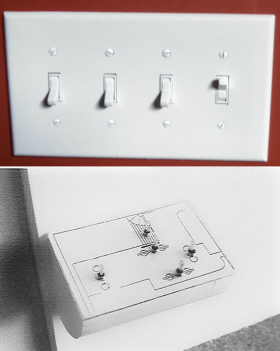
\includegraphics[scale=0.75]{interuttori.png}\\
\columnbreak

Vincoli e mapping alle volte si confondono fra loro. Nell'esempio, posizionare gli interuttori in corrispondenza delle luci sulla piantina della stanza è un mapping così forte che è quasi un vincolo logico: non ti puoi permettere di sbagliare interuttore.
\end{multicols}
\subsection{Forcing functions}
\textbf{Forzare le funzioni} è una forma di \textbf{vincolo fisico}.\\\\
\textbf{Interlock}: azione \textbf{dopo serie di passi}\\
\textbf{Lock-In}: azione \textbf{prima di concludere}\\
\textbf{Lock-Out}: azione \textbf{prima di iniziare}
\subsubsection{Interlock}
L'\textbf{interlock} consiste nell'\textbf{obbligare l'utente ad eseguire una successione di azioni} per raggiungere un certo stato/obiettivo (ad esempio premere pedale e due pulsanti distanti per azionare una pressa idraulica) oppure anche per guidare il learning (ad esempio un tutorial).
\paragraph{Esempi} "\textit{Verifica la tua mail}" prima di poter accedere con un account appena creato.
\subsubsection{Lock-In}
Con un \textbf{lock-in} invece \textbf{metto in pausa l'attuale situazione fino a che l'utente non ha fatto una determinata cosa}. 
\paragraph{Esempi} Non puoi uscire dall'editing di un documento se consciamente non mi hai detto di salvarlo o buttarlo.\\\\
A volte una lock-in \textbf{funziona così bene che diventa una shortcut}: chiudo e uso la finestrella di lock-in per salvare, invece di andare col mouse a premere tasto in alto a sinistra.
\subsubsection{Lock-Out}
Una \textbf{lockout} è l'opposto della lock-in, cioè \textbf{chiude fuori l'utente finché non compie una determinata azione}
\paragraph{Esempi} Finestra \textit{v.m. 18}, assolve alla richiesta legale di vietare l'accesso ai minorenni. Io utente posso \textbf{dichiarare il falso} ed entrare comunque, ma così il reato l'ho fatto io e non il sito.
\subsection{Activity-Centered Controls}
In molti casi è comodo avere \textbf{controlli associati alle attività} piuttosto che alle funzioni.\\Particolare modalità di interazione utente che usa tutti i principi precedentemente elencati.
\paragraph{Un esempio} Invece di avere un pulsante "\textit{abbassa telo}", un altro pulsante "\textit{alimenta proiettore}", un altro "\textit{accendi proiettore}" e così via, posso fare un pulsante "\textit{\textbf{presentazioni con slide}}" che esegue tutte quelle operazioni.\\Altro esempio sono i preset per le impostazioni di schermi e audio: si possono ottenere i medesimi risultati manualmente. Il preset lo rende semplicemente più veloce.
\paragraph{Teoria vs Pratica} Nella teoria le activity-centered controls sono eccellenti, ma nella pratica sono difficili da costruire bene. Se fatte male, creano \textbf{difficoltà}. Per questo \textbf{le activity-centered controls devono essere disegnate sugli utenti} e non sullo sviluppatore.\\
L'elettricista programmerà il pulsante "\textit{presentazioni con slide}" \textbf{con la sua idea} di presentazione: probabilmente questa idea sarà super completa ma \textbf{talmente specifica che non andrà bene a nessun utente}. Invece \textbf{bisogna fare user activity-centered control}: tutta la parte sullo HCD si applica anche qua, cioù chiedersi chi è l'utente, le sue caratteristiche e così via. Ciò deve portare a \textbf{creare quella scena di presentazione che abilita tutti gli utenti}. Eventualmente per qualcuno andrà bene così com'è, mentre per un altro potrebbe essere incompleta e premerà altri pulsanti.\\\\
Un altro errore comune è creare un'apparente activity-centered control ma in realtà creare device-centered control.
\section{How People do Things}
\paragraph{Come fanno le persone a fare cose?} \textbf{Finchè le cose vanno bene allora sembrano essere semplici}, l'utente crede di aver chiaro come ha ottenuto un risultato e allo sviluppatore sembra chiaro come l'utente esegue le attività.\\
Invece, \textbf{quando le cose vanno male allora l'interpretazione è opposta}, cioè l'utente non capisce perché siano andate male e diventa frustrato: questo accade perché \textbf{il modo in cui le persone fanno le cose è complesso}. I fenomini mentali in atto quando si fanno le cose sono complessi.\\
\textbf{Quando le cose vanno bene non ce ne rendiamo conto}, ma \textbf{quando ci sono problemi ce ne rendiamo conto \textit{in una serie di fasi}}, che sono le fasi eseguite durante l'ottenimento di un obiettivo.
\paragraph{Come ottenere un obiettivo} Si dà per scontato che le persone eseguano delle azioni, ma \textbf{prima di tutto persone scelgono le azioni da compiere}. Si dà per scontato che l'utente scelga l'azione scelta dal progettista.
\subsection{I Golfi}
\begin{multicols}{2}
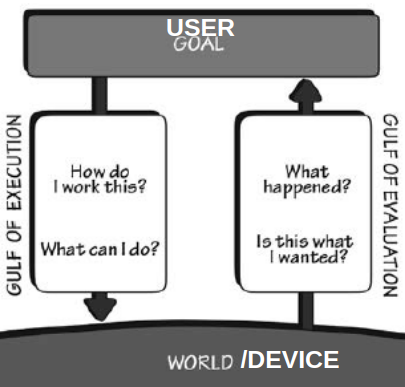
\includegraphics[scale=0.6]{golfi.png}
\columnbreak


Immagino l'\textbf{utente} e il \textbf{mondo fisico/device} contrapposti. Considero due "flussi": quello dell'\textbf{esecuzione} di una serie di attività e quello della \textbf{valutazione} della risposta ottenuta dal sistema.\\
I due flussi vengono descritti come due \textbf{golfi}, seguendo l'analogia che \textbf{tanto più profondo è un golfo tanto più lunga è la strada da percorrere per giungere dall'altra parte}.
\begin{list}{-}{}
\item Nel \textbf{golfo dell'esecuzione} gli utenti cercano di capire cosa fare e, una volta capito, eseguono le azioni
\item Nel \textbf{golfo della valutazione} l'utente interpreta e valuta il feedback ricevuto dal sistema
\end{list}
Il golfo della valutazione è ritenuto dai designer il più semplice da superare. Nel golfo della valutazione c'è una quantità di effort mentale che l'utente usa per comprendere l'interfaccia e capire se l'azione che aveva deciso di fare è stata eseguita come da lui pianificato. \textbf{Tanto più il modello mentale differisce} da quello concettuale, \textbf{tanto più il golfo valutazione sarà grande}.
\end{multicols}
\paragraph{Mitigare} Gli elementi del design che contribuiscono alla mitigazione del \textbf{golfo dell'esecuzione} sono: \textbf{significanti}, \textbf{constraint}, \textbf{mapping} e \textbf{modello concettuale}.\\
Gli elementi che contribuiscono a alla mitigazione del \textbf{golfo della valutazione}: \textbf{feedback} e \textbf{modello concettuale}.
\paragraph{Fare ed Interpretare} Le \textbf{due parti di un'azione} sono: \textbf{fare} l'azione e \textbf{valutare} i risultati. In entrambe le parti bisogna \textbf{garantire l'understanding}, cioè la \textbf{discoverability} e la \textbf{visibility}: ad esempio se non so quando ottengo punti ma vedo aumentarli apparentemente a caso non posso capire perché li ottengo se non è facilmente discoverable.
\subsection{Sette Stati dell'Azione}
\begin{multicols}{2}
Sono i sette stati attraverso i quali passano i due golfi:\\
Per prima cosa \textbf{(1)} si \textbf{specifica il proprio obiettivo}. Dopodiché si passa ai 3 stati dell'esecuzione:
\begin{list}{}{}
\item \textbf{2}: \textbf{Pianifico} ciò che devo fare
\item \textbf{3}: \textbf{Specifico} la mia pianificazione in task
\item \textbf{4}: \textbf{Eseguo} i vari task pianificati: click del pulsante, riempimento dei campi...
\end{list}
Anche la valutazione ha 3 stati:
\begin{list}{}{}
\item \textbf{5}: \textbf{Percepisco} cosa è accaduto (il feedback)
\item \textbf{6}: \textbf{Interpreto} ciò che ho percepito. Non è detto che io abbia lo strumento corretto per interpretare o che il feedback sia sufficiente da essere interpretato
\item \textbf{7}: \textbf{Comparo} il risultato dell'interpretazione con il mio obiettivo, che non devono differire
\end{list}
\columnbreak


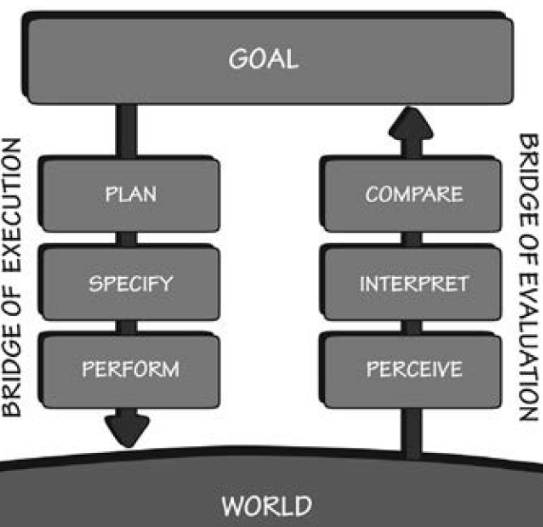
\includegraphics[scale=0.45]{settestatiazione.png}
\end{multicols}
\begin{center}
\texttt{Goal $\rightarrow$  Plan $\rightarrow$ Specify $\rightarrow$ Perform $\rightarrow$ Percieve $\rightarrow$ Interpret $\rightarrow$ Compare}\\
\end{center}
Non è detto che tutti i comportamenti debbano passare da tutte le fasi sopra descritte. Per esempio, l'abitudine porta ad abilitare altre parti cervello e non rende più necessaria la specify o consente di saltare la pianificazione, perché al goal associo già la sequenza di azioni più veloce che conosco già.\\
Un'altra situazione è il caso in cui il feedback non si possa comparare al goal, che quindi abilita nuovo processo. Per esempio quando vado a concludere un acquisto ma non sono registrato, il feedback è "inserisci i dati per la registrazione" che non è compatibile con il mio obiettivo "acquista prodotto" $\rightarrow$ Inizia un nuovo processo)\\
Il trucco è sviluppare delle skill per utilizzare questo pardigma di analisi interazioni per capire se le nostre interfaccia performano bene o no.
\pagebreak
\subsubsection{Tre livelli di Processing}
\begin{multicols}{2}
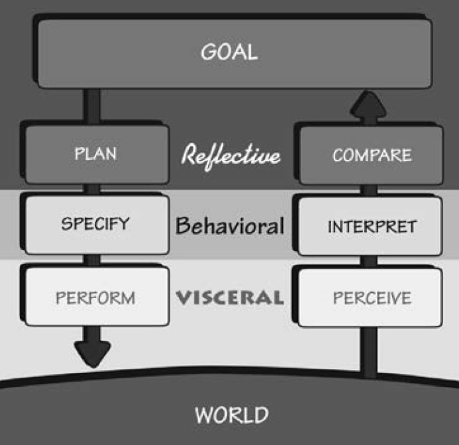
\includegraphics[scale=0.5]{treprocessing.png}

\begin{list}{}{Gli stati dell'azione possono essere associati con tre livelli di processing mentale:}
\item \textbf{Viscerale}: \textbf{comportamento basilare}, istantaneo e quasi del subconscio. \textit{Clicco qua, vedo lo schermo}.
\item \textbf{Comportamentale}: guidato dalle \textbf{aspettative} durante l'esecuzione e guidato dalle emozioni durante l'attesa di conferma di tali aspettative. \textbf{Decide in che modo faccio} un determinato task e \textbf{in che modo interpreto} un determinato feedback.
\item \textbf{Riflessiva}: relativo alle emozioni, che valuta i risultati in termini di presunti agenti causanti e le loro conseguenze. Essendo la \textbf{parte più emotiva}, è qui che avviene la soddisfazione e l'orgoglio, ma anche la frustrazione e il senso di colpa.
\end{list}
\end{multicols}
\section{Sette Principi Fondamentali della Progettazione}
\subsection{Sette Domande}
\begin{multicols}{2}
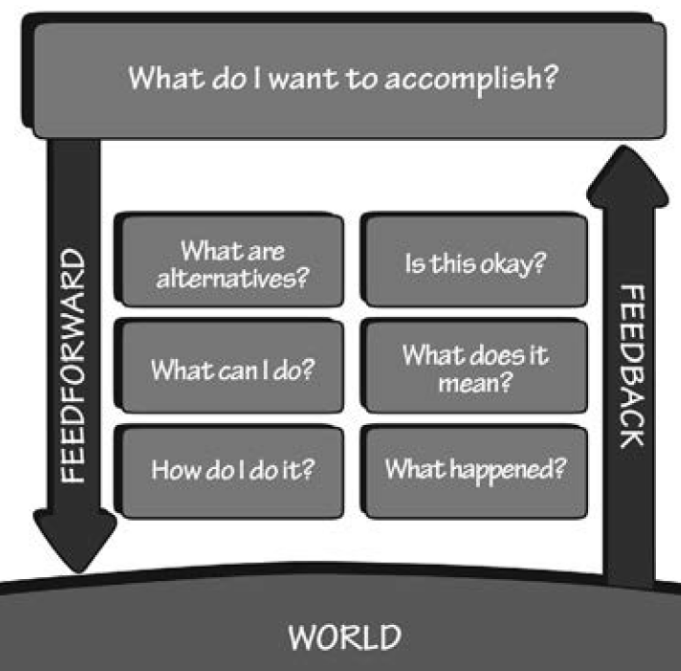
\includegraphics[scale=0.345]{setteprincipi.png}

\columnbreak
Il modello dei sette stati dell'azione può essere un utile strumento di progettazione, poiché \textbf{fornisce una checklist basilare di domande da porsi} durante il design. In generale, \textbf{ogni stato dell'azione richiede strategie di design specifiche} e offre le proprie opportunità di disastro.
\begin{list}{-}{Derivano quindi 7 domande, a cui \textbf{dovrebbe poter rispondere chiunque} stia usando quel prodotto.}
\item \textbf{Cosa voglio ottenere?}\\Ad esempio, dalle personas individuate genero come obiettivo "\textit{voglio selezionare le scarpe divise per modello}" $\rightarrow$ vedo che nell'interfaccia non ho inserito la scelta per modello.
\item \textbf{Quali sono le sequenze d'azione alternative} che posso compiere per raggiungere comunque l'obiettivo?
\item \textbf{Che azione posso fare ora?}
\item \textbf{Come posso fare quest'azione?}
\item \textbf{Cosa è successo?}
\item \textbf{Cosa significa?}
\item Va bene? \textbf{Ho raggiunto il mio obiettivo?}
\end{list}
\end{multicols}
\pagebreak
\subsection{Feedforward e Feedback}
\paragraph{Feedforward} Tutta l'informazione che aiuta a rispondere alle domande riguardo l'esecuzione, quindi l'insieme di affordances, significanti e mapping.
\paragraph{Feedback} Tutta l'informazione che aiuta a \textbf{capire cos'è successo, macchina $\rightarrow$ uomo}\\\\
Feedback e feedforward vengono realizzati correttamente attraverso i \textbf{sette principi di design}. Occorre far notare che i sette principi non sono mappati uno ad uno con i sette stati del processo d'interazione: il fatto che siano entrambi \textit{sette} è una casualità, non perché sono correlati. I sette principi costituiscono una "\textit{checklist da fare prima del commit}".
\subsection{Sette Principi}
\begin{enumerate}
\item \textbf{Discoverable}: il design deve \textbf{mettere utente nella posizione di capire cosa può fare} e capire lo stato del dispositivo con cui interagisce
\item \textbf{Feedback}: un sistema che dà feedback sbagliati, non esplicativi, in ritardo, che annoiano ecc. è un sistema che ha problemi. Deve esserci un flusso continuo di informazione sui risultati delle azioni e sullo stato attuale del prodotto/servizio: \textbf{deve essere facile determinare il nuovo stato dopo aver compiuto un'azione}.
\item \textbf{Modello Concettuale}: il modello concettuale che ho pensato è percepibile? Regge? Lo capisco solo io o tutti? Il \textbf{design deve proiettare tutte le informazioni necessarie a passare il corretto modello} all'utente.
\item \textbf{Affordances}: il dispositivo/interfaccia abilità la proprietà dell'interazione \textbf{con le categorie di utenti con cui sto lavorando}. L'affordances \textbf{esiste laddove è percepibile}, se non so se lo schermo è touch o no potenzialmente per me l'affordances non esiste.
\item \textbf{Significanti}: importanti perché \textbf{se usati bene abilitano la discoverability funzionalità} e la corretta percezione ed interpretazione dei feedback.
\item \textbf{Mapping}: ho messo significante che va contro le capacità mentali utente? Un buon mapping è quello naturale.
\item \textbf{Constraint}: usati con parsimonia, posizionare vincoli fisici, logici, semantici e culturali \textbf{guida le azioni e facilita l'interpretazione}
\end{enumerate}
Con questi sette principi si conclude la parte dedicata a strumenti, metodi ed elementi per il design dello human-computer interaction.\\
\subsection{Opportunismo}
Non sempre gli utenti eseguono delle azioni deliberatamente pianificate, ma alle volta eseguono \textbf{azioni di tipo opportunistico}.\\L'opportunismo \textbf{rompe} lo schema d'interazione Obiettivo $\rightarrow$ Mondo.
\paragraph{Azioni opportunistiche} Queste azioni sono quelle in cui il \textbf{comportamento scaturito dalle circostanze prevale sulle pianificazione} e quindi su modo di essere, di conseguenza \textbf{prevarica tutto il discorso precedente}.\\\\Ci sono quindi situazioni in cui può accadere che abbia progettato tutto bene seguendo i principi, ma l'utente non si comporta in un modo che avevo previsto. Questo \textbf{può succedere}, perché gli \textbf{utenti agiscono in maniera incontrollata specialmente se guidati dalle opportunità}.
\section{Disruptive Innovation}
La \textbf{maggior parte dell'innovazione è fatta migliorando incrementalmente prodotti già esistenti}. La \textbf{disruptive innovation} invece riguarda le \textbf{idee radicali}, cioè l'\textbf{introdurre nuove categorie di prodotto nel mercato}.
\paragraph{Innovazione Lineare} Si migliora il sistema esistente: abbasso i consumi, miglioro l'efficienza\ldots
\paragraph{Disruptive Innovation} Si tratta più di un cambio di binario.\\Ad es. prima si guardavano i film andando fisicamente a prenderli a noleggio, mentre adesso basta accedere ad un catalogo già "presente nel nostro televisore". \textbf{Cambia il modello di business}. Ciò che nasce da un processo disruptive tipicamente fa fallire i metodi di business classici.\\
"\textit{La gente non vuole un trapano di 5 millimetri, vuole un buco di 5 millimetri}" -- Theodore Levitt
\paragraph{Metodi} Ci sono dei metodi per arrivare alla disruptive innovation, non la si "sogna". Il cliente del nuovo modello di sistema e di business non è tipicamente conosciuto, così come il mercato: impossibile eseguire la user experience analysis.
\subsection{Root Cause Analysis}
Una volta che si è capito che l'utente non vuole il trapano, magari ci si accorge che \textbf{non vuole nemmeno un buco} ma \textbf{vuole installare la libreria}: \textbf{perché non sviluppare metodi che non richiedono buchi nel muro?} O ancora, \textbf{libri che non richiedono librerie}?\\
La \textbf{RCA} è, letteralmente, l'analisi dell'origine delle cause. La gente non vuole uno scaffale ma desidera un \textbf{modo per contenere i libri} $\longrightarrow$ e-Book Reader.\\
Si pensa a \textbf{cosa fa} l'utente e \textbf{perché lo fa}, non per migliorare il libro. Il libro è un contenitore di testo.\\
Nella \textbf{disruptive innovation} viene \textbf{scomposta la RCA}.
\subsubsection{Why root cause analysis}
Il processo di RCA più tipico, nel quale \textbf{non ci si ferma a dire cosa è successo, si vanno a comprendere le cause alla base del perché è capitato}.\\
La root cause analysis produce la \textbf{task analysis}: la RCA produce la \textbf{serie di attività} (task) da eseguire per raggiungere un obiettivo.\\
Questa analisi può essere suddivisa in 4 passaggi:
\begin{enumerate}
\item \textbf{Identificare e descrivere} chiaramente il problema.\\
Ad esempio: spostare le persone da un punto A ad un punto B
\item \textbf{Creare una timeline} che porti \textbf{sequenzialmente} dalla identificazione del bisogno al suo compimento.\\
Chiamo taxi $\rightarrow$ aspetto $\rightarrow$ si ferma $\rightarrow$ entro $\rightarrow$ dico la destinazione $\rightarrow$\ldots
\item \textbf{Distinguere le vere cause} (root cause) dai fattori collaterali.\\
Non c'entra la dimensione della pensilina d'attesa, è un problema locale.
\item \textbf{Creare un grafico di causa-effetto} tra il problema e la root cause
\end{enumerate}
\paragraph{Perché serve?} Avere una struttura così solida aiuta a discutere in azienda, in team\ldots, idee su come innovare. Si discute sulla forma e sul metodo ma non su come andare dal punto A al punto B. \textbf{Questo aspetto unico per tutti va scritto}.\\
I task estratti sono di \textbf{tipo utente} e \textbf{non tecnologico}, si parla della \textbf{user experience}. La task analysis è il processo di apprendimento di un fenomeno fatto tramite l'esperienza, l'\textbf{osservazione di come sono eseguite le attività in esame}.\\


\pagebreak
Si consiglia di \textbf{estrarre più task e il più dettagliati possibile} al fine di:
\begin{list}{}{}
\item \textbf{Comprendere} nel profondo gli \textbf{obiettivi}
\item \textbf{Cosa fanno} gli utenti \textbf{per raggiungere} quell'\textbf{obiettivo}
\item \textbf{Quale esperienza} (personale, sociale, culturale\ldots) l'\textbf{utente porta} all'attività
\item \textbf{Come} gli utenti \textbf{sono influenzati dall'ambiente circostante}
\item \textbf{Quali conoscenze ed esperienze precedenti influenzano}
\begin{list}{}{}
\item ciò che pensano del loro operato
\item la sequenza di attività che seguono per portare a termine le proprie attività
\end{list} 
\end{list}
\subsubsection{Tipi di Task Analysis}
Ci sono \textbf{due metodi} che danno \textbf{due tipologie} di task analysis:
\begin{list}{}{}
\item \textbf{Cognitive} task analysis: concentrata sul capire i task che richiedono \textbf{decision-making}, \textbf{problem-solving}, \textbf{memoria}, \textbf{attenzione} e \textbf{giudizio}
\item \textbf{Hierarchical} task analysis: butto giù dei macro-task e li scompongo in sotto-task
\end{list}
\subsubsection{Come fare la Task Analysis}
Il processo per decomporre task di alto livello segue i seguenti passi
\begin{enumerate}
\item \textbf{Identifica} il task da analizzare
\item \textbf{Scomponi} questo task in \textbf{4--8 sottotask}.\\
I sottotask dovrebbero essere specificati in termini di obiettivo e, tra tutti, \textbf{coprire l'intera area d'interesse}.
\item Disegna un \textbf{diagramma a strati} per ogni sottotask, assicurandoti che sia completo
\item Scrivi un resoconto e la decomposizione del diagramma
\item \textbf{Presenta l'analisi a qualcuno} che non sia stato coinvolto nella decomposizione ma che conosca l'attività abbastanza bene da verificarla.
\end{enumerate}
\subsubsection{Livello di dettaglio}
\paragraph{Quando mi fermo?} Non c'è una risposta, è un'arte. Non c'è un metodo o una formula. Richiede esperienza e buonsenso.\\
Sarebbe bene \textbf{definire un criterio di arresto}, anche se all'inizio non si hanno gli strumenti per farlo. Agli inizi è meglio realizzare un'analisi più dettagliata possibile, poiché no esperienza sull'eliminare.
\section{Agile}
\begin{quote}
"\textit{Design thinking è come esploriamo e risolviamo i problemi;\\Lean è il nostro framework per testare le nostre idee e imparare a ottenere gli obiettivi;\\
e Agile è come ci adattiamo ai cambiamenti nelle condizioni del software."}
\end{quote}
\paragraph{Non un semplice framework} Si pensa che l'Agile sia semplicemente uno strumento di sviluppo, ma in verità l'\textbf{Agile è un modo di pensare} alla stregua del design thinking, fa parte della famiglia dei metodi di lavoro.
\begin{list}{}{}
\item Il \textbf{design thinking} è \textbf{come ci poniamo nella soluzione dei problemi}
\item l'\textbf{Agile} è \textbf{come applichiamo i metodi del design thinking allo sviluppo software}.
\end{list}
L'\textbf{Agile è una forma mentis}, poi ad esempio lo scrum è una tecnica di organizzazione team \textbf{di tipo Agile}.
\paragraph{Individui} Il \textbf{focus è sugli individui e l'interazione} (programmatori) invece che sui processi e sui tool (di sviluppo)\\
\textbf{Software funzionante} invece di grandi documenti\\
Capacità di \textbf{adattamento} al cambiamento.
\subsection{12 principi dell'agile}
\texttt{https://www.agilealliance.org/agile101/the-agile-manifesto/}\\
Il \textbf{concetto più importante} è quello della \textbf{adattabilità}. La mancanza di struttura e di documenti \textbf{non è anarchia}, \textbf{anzi è molto complesso} garantire al resto del team di aver compiuto qualcosa che non penalizzi i colleghi, in assenza di un "grande capo" che controlla la produzione.
\subsection{Personas}
% [7] Personas, scenarios, user stories and storyboards, 8
Identificato correttamente e precisamente il problema (dalla \textbf{task analysis}), come creo gli elementi individuali?
\paragraph{Identificare le personas} Il primo passo da fare dopo aver concluso la task analysis è \textbf{identificare le personas}.\\
Una \textbf{personas} è l'\textbf{archetipo di uno dei nostri utenti}: \textit{la casalinga di voghera}, l'\textit{utente anziano}, l'\textit{infante}. Identifichiamo le personas subito dopo la task analysis \textbf{perchè durante di essa ci si rende conto che non tutti si comportano nello stesso modo}. Si rende \textbf{necessario creare degli archetipi}. Durante la macro task analysis, quindi, posso appuntarmi delle note da cui poi genero le personas.
\paragraph{Debugging} Nel produrre le personas si \textbf{innesca un processo} durante il quale, \textbf{mentre scrivo} le \textbf{personas}, \textbf{affino} la \textbf{task analysis}.
\paragraph{Mettersi nei panni dell'utente} Definire le personas mette a fuoco la userbase e \textbf{colma la distanza tra azienda e cliente}. Questo \textbf{perché ci si prova a immedesimare in un archetipo dei potenziali clienti, descrivendone la figura}. Questo è l'\textbf{unico modo per provare davvero a capire l'utente}.
\subsubsection{Scrivere le personas} Creare una personas tipicamente parte dalla \textbf{user research}: come la task analysis, ci sono altre metodologie a partire dai \textbf{feedback} (questionari e focus group) fino ai \textbf{prototipi}, cioè sperimentando con le idee prima di svilupparle. Tipicamente le personas sono caratterizzate da un \textbf{goal}.
\subsubsection{Quante personas scrivere?} Uno dei principi fondamentali al mondo è il \textbf{Principio di Pareto}: \textit{l'80\% degli effetti è generato dal 20\% delle cause}.\\
Anche la progettazione delle personas dovrebbe seguire questo principio. Bisogna concentrarsi sul \textbf{20\% della userbase che userà/comprerà l'80\% delle funzionalità/prodotti o che sarà responsabile dell'80\% degli introiti}.
\subsection{Requirements}
Un \textbf{requirement} è \textbf{una peculiarità} (proprietà, serivzio, funzione\ldots) \textbf{che il mio sistema deve avere al fine di assolvere al need dell'utente}.
\begin{center}
\emph{Persona $\Rightarrow$ Need $\Rightarrow$ Requirement}
\end{center}
Oltre a funzionalità \textbf{possono anche essere dei costraints}: un utente minorenne ha come requirement un costraint su certi siti che richiedono un lockout.
\paragraph{Lavoro complesso} Scrivere requirements è molto \textbf{complesso}, oneroso e va \textbf{in contrasto col metodo Agile}: si richiede di \textbf{essere sempre pronti al cambiamento}, ma se faccio requirement-driven development si rischia di essere invece poco flessibili, per questo i \textbf{requirement stanno uscendo di moda}.
\pagebreak
\subsubsection{Tipi di requirement} I requirement sono divisi in:
\begin{list}{}{}
\item \textbf{Functional Requirements} o FR: i requirement \textbf{funzionali} esprimono una \textbf{funzione o funzionalità che il sistema deve avere}. \textbf{Non esprimono come deve essere fisicamente ottenuta una soluzione}.\\
Esempi: \textit{ottenere lo storico degli ordini}, \textit{accedere al sito del cliente}\ldots\\
Entrambi possibili in tanti modi, con database, link ipertestuali, frame embedded ecc.
\item \textbf{Non-Functional Requirements} o NFR: i requirement \textbf{non funzionali} definiscono \textbf{quanto bene, o a quale livello, una soluzione deve comportarsi}. Sono i cosiddetti \textbf{vincoli di qualità}: legislativi, di efficienza, sicurezza, formato\ldots Descrivono quindi \textbf{gli attributi di una soluzione}.\\
Esempi: \textit{rispondere entro 2 secondi}, \textit{essere conforme alla GDPR}\ldots
\end{list}
\subsection{User Stories}
Il prossimo passo è \textbf{la scrittura delle user stories}. 
\paragraph{Cosa sono} Una \textbf{user story} è una \textbf{breve descrizione che identifica l'utente insieme al suo obiettivo}. Determina \textbf{chi è l'utente}, di \textbf{cosa ha bisogno} e \textbf{perché ne ha bisogno}.\\
Tipicamente c'è \textbf{una o più user story per personas}, \textbf{non ci possono essere più personas per user story} -- significherebbe l'aver introdotto troppe personas.\\
Se una user story non copre tutte sfaccettature della singola personas allora dovrei suddividere tale personas, perché forse ho definito una personas troppo ampia.\\\\
Una \textbf{user story è un requirement espresso dalla prospettiva dell'utente}.
\paragraph{Debugging} Definire le user stories aiuta a \textbf{migliorare le personas}.
\subsubsection{Come scrivere le user stories}
Scrivere una user story è molto semplice
\begin{center}
\emph{As a <role>, I want <feature> because <reason>.}
\end{center}
I vare elementi sono presi dalla personas in esame. Notare che il role non è per forza la personas in esame, ma \textit{potrebbe} esserlo.
\paragraph{Chi scrive le user stories} \textbf{Chiunque} può scrivere le user stories. Nonostante sia responsabilità del product owner assicurarsi che siano definite le user stories, ciò non significa che sia necessariamente compito suo scriverle.\\
Durante lo sviluppo di un buon progetto Agile, \textbf{ogni membro del team} dovrebbe produrre una user story.\\
Inoltre, \textbf{chi scrive la user story è molto meno importante rispetto a chi è coinvolto nella sua discussione}.
\paragraph{Livello di dettaglio}
Uno dei vantaggi delle user stories è che \textbf{possono essere scritte a livelli di dettaglio variabili}. Si possono scrivere user stories che coprono ampi aspetti delle funzionalità, e sono chiamate \textbf{epics} o epiche.\\
Un esempio di \textbf{epic agile user story} di un software per backup: "\textit{As a user, I can backup my entire hard drive.}"
\paragraph{Come aggiungere il dettaglio}
Poiché una epic è solitamente \textbf{troppo grande per essere completata in una iterazione} da un team Agile, viene solitamente \textbf{divisa in user stories più piccole} prima di iniziare a lavorarci.\\
L'epica precedente può essere suddivisa in dozzine, o addirittura centinaia, di altre user stories, tra cui:
\begin{list}{}{}
\item "\textit{As a power user, I can specify files or folders to backup based on file size, date created and date modified.}
\item "\textit{As a user, I can indicate folders not to backup so that my backup drive isn't filled up with things I don't need saved.}"
\end{list}
\pagebreak
Il \textbf{dettaglio} può \textbf{essere aggiunto ad una user story in due modi}:
\begin{list}{}{}
\item \textbf{Suddividendo} una user story in diverse user stories più piccole.\\
Quando una user story relativamente grande viene suddivisa in diverse user stories più piccole, viene naturale pensare che si sia aggiunto dettagglio. Dopotutto, si è scritto di più.
\item \textbf{Aggiungendo} "condizioni di soddisfacimento".\\
Le \textbf{condizioni di soddisfacimento} sono semplicemente test di accettazione ad alto livello che saranno verificati dopo che la user story è completa.
\end{list}
"\textit{As a vice president of marketing, I want to select a holiday season to be used when reviewing the performance of past advertising campaigns so that I can identify profitable ones.}"\\
Posso \textbf{aggiungere dettaglio} a questa user story \textbf{aggiungendo le seguenti condizioni} di soddisfacimento:
\begin{list}{-}{}
\item Assicurarsi che funzioni con le festività più importanti: Natale, Pasqua, Festa della Mamma\ldots
\item Supportare feste che avvengono a cavallo di due anni
\item \ldots
\end{list}
\subsection{Scenarios}
Uno \textbf{scenario} è l'\textbf{evoluzione delle user stories}.\\
Con una user story \textbf{sintetizzo in brevi frasi associate alle personas ciò che tali personas fanno con il mio software}. Lo scenario \textbf{estende a partire da questo}: inizia a catturare anche \textit{come} l'utente si comporterà sul sistema. Questo "come" non è da intendersi nell'accezione dei task spacchettati, ma  \textbf{più in generale}. Inoltre permangono i goal delle personas e li si estendono, venendo \textbf{descritti in maniera più ampia}. Gli scenario sono poi \textbf{divisi in singoli use case}.
\paragraph{A cosa servono?} Le user stories sono sintetiche, brevi e dicono cosa sviluppare. Gli scenarios invece sono \textbf{utili per interloquire con gli stakeholder}. Questo perchè \textbf{per gli esterni} al progetto \textbf{le user stories non sono facilmente comprensibili}. Al contrario, gli scenarios \textbf{convogliano immediatamente l'immagine dell'obiettivo}.\\
Gli scenarios diventando quindi \textbf{fondamentali per allinearsi con le richieste del cliente}. Senza di essi si rischia di presentare un progetto finito senza che il cliente sia soddisfatto, poiché le user stories che avevamo definito non confluivano nel risultato che il cliente si auspicava. \textbf{Una volta approvati} gli scenario \textbf{ho raggiunto metà dell'opera}: non ho fissato i requirements, quindi \textbf{sono ancora flessibile agli eventuali cambiamenti}, e il \textbf{software che realizza gli scenarios approvati sarà sicuramente soddisfacente per il cliente}, perché \textbf{gli scenarios sono stati approvati da lui stesso}.
\subparagraph{Stakeholder} Colui che è interessato all'output del progetto: cliente, capo, project manager\ldots
\subsubsection{Cosa tenere in considerazione}
Un buon scenario è \textbf{conciso ma risponde alle seguenti domande chiave}:
\begin{enumerate}
\item \textbf{Chi è l'utente?} Usa le personas sviluppate\\Es: \textit{il tecnico}
\item \textbf{Qual è la motivazione che lo ha spinto ad arrivare da me?} Cosa motiva l'utente ad arrivare al mio sistema e le sue aspettative all'arrivo\\Es: \textit{perché sono un sistema che fa report automatico}
\item \textbf{Qual è il suo obiettivo?} Attraverso la task analysis, puoi comprendere meglio cosa voglia l'utente dal tuo sistema, quindi cosa deve avere il sistema per soddisfare l'utente\\Es: \textit{fare report automatico}
\end{enumerate}
\textbf{In alcuni casi} uno scenario potrebbero includere aspetti di \textbf{come} fare cose, ma ciò appartiene al mondo degli \textbf{use case}. Sono preferibili scenarios privi di tale aspetto.
\pagebreak
\subsubsection{Come scrivere uno scenario}
Prima di iniziare a definire gli scenario, è necessario \textbf{mapparli}. Bisogna partire avendo già le personas e le relative user stories, e individuare per ogni personas un \textbf{key task} che tale personas vuole ottenere.\\
\textbf{Scrivo gli scenarios racchiudendo una o più user stories relative alla personas}. Tipicamente \textbf{per ogni personas descrivo almeno uno scenario}.
\paragraph{Focalizzarsi sul key task} Il \textbf{key task} diventa il task \textbf{fondamentale di quello specifico scenario}, ad esempio \textit{l'utente che compra il biglietto}.\\
Gli scenarios quindi \textbf{contestualizzano i goal dell'utente}: il mio goal è \textbf{comprare il biglietto}, lo contestualizzo sul mobile, desktop, tablet, biglietteria\ldots
\paragraph{Mindset} Sviluppare gli scenarios richiede un \textbf{mindset dedicato} a risolvere questo problema. Nella scrittura di uno scenario è importante \textbf{riuscire a esprimere qual è il goal dell'utente e com'è influenzato dal contesto dello specifico utente}, dalla \textbf{prior knowledge} e dal \textbf{background} -- evincendo ciò dalla personas.\\\\
Gl scenarios portano quindi le user stories al livello successivo e sono relativi all'\textbf{esperienza della personas}, \textbf{integrando con l'interazione che avviene tra l'utente e il prodotto o il servizio} della story.\\\\
\texttt{https://uxknowledgebase.com/scenarios-43e05671b07}
\subsubsection{Tre metodi} Ci sono tre metodi principali per scrivere gli scenarios\\(\texttt{https://www.usability.gov/how-to-and-tools/methods/scenarios.html}):
\begin{enumerate}
\item \textbf{Goal}/\textbf{Task Oriented}
\item \textbf{Elaborated Scenarios}
\item \textbf{Full Scale Task Scenarios}: da evitare poché diventano del tutto uguali agli use cases.
\end{enumerate}
Conviene \textbf{partire scrivendo uno scenario goal/task-oriented} e \textbf{aggiungendo elementi di contesto}.
\paragraph{Ricapitolando} Parto dall'estensione di un paio di user stories.\\
Percorso di debug a partire dall personas $\rightarrow$ trovo elementi di contesto o particolarità da aggiungere.\\
Senza troppo dettaglio.
\subsection{Use Cases}
Gli \textbf{use cases} sono l'\textbf{evoluzione degli scenarios}. In uno \textbf{use case ho la narrativa, in step monolitici}, che partono dall'obiettivo dell'utente e finiscono ad obiettivo raggiunto, \textbf{del comportamento del sistema in risposta alle richieste} visto dal punto di vista dell'utente.\\
Essendo una serie di step monolitici, gli use case \textbf{sono nuova task list}, \textbf{prodotta dal processo di design} per innovare un metodo visto e descritto in precedenza tramite la task analysis.
\paragraph{Un attore} Uno scenario si concentra su una situazione. \textbf{lo use case} invece \textbf{è incentrato sulla personas}: \textit{John e le cose che fa}. \textbf{Uno scenario si trasforma in un set di use case}.\\
La differenza principale è la \textbf{prospettiva}.\\\\
Esempio di scenario: \textit{voglio ritirare una somma dal bancomat}\\
Use Case relativi: \begin{list}{-}{}
\item \textit{Cliente della banca che possiede lo sportello}
\item \textit{Cliente di un'altra banca}
\end{list}
\paragraph{Diretti allo sviluppo} Gli use case sono di fondamentale importanza perché \textbf{vanno direttamente al team di sviluppo}. Con degli use case ben fatti lo sviluppo è molto pià facile e si riduce a semplice implementazione, poiché \textbf{ho già delineato precisamente cosa deve fare il sistema}, fornendo una lista di obiettivi che può essere usata anche per stabilire costo e complessità del sistema. Si può quindi anche negoziare quali funzioni entraranno effettivamente in sviluppo.
\subsubsection{Elementi}
\begin{multicols}{2}
\begin{list}{}{\textbf{Cosa è incluso} in uno use case}
\item L'utente
\item Cosa vuole fare
\item Qual è il goal finale
\item I singoli step necessari
\item I feedback del sistema durante gli step
\end{list}
\columnbreak

\begin{list}{}{\textbf{Cosa non è incluso} in uno use case}
\item Qualsiasi dettaglio implementativo e di scelta tecnologica, che non sia un costraint o un requirement
\item Dettagli a proposito dell'interfaccia utente
\end{list}
\end{multicols}
A seconda di quanto livello di dettaglio si desidera raggiungere, gli use case descrivono una combinazione dei seguenti elementi
\begin{list}{}{}
\item \textbf{Attore} -- Chiunque o qualsiasi cosa che esegue un comportamento (che sta usando il sistema)
\item \textbf{Stakeholder} -- Qualcuno o qualcosa interessato al comportamento del sistema
\item \textbf{Attore Primario} -- Stakeholder che inizia l'interazione con il sistema per raggiungere un obiettivo
\item \textbf{Pre/postcondizioni} -- Cosa deve essere verificato o deve succedere prima e dopo l'esecuzione dello use case
\item \textbf{Triggers} -- Gli eventi che scatenano lo use case
\item \textbf{Basic Flow} -- La \textbf{sequenza principale degli eventi}, ovvero la sequenza di azioni nel caso in cui niente vada storto
\item \textbf{Alternative Flow} -- La \textbf{sequenza alternativa degli eventi}, sequenze di azioni che variano la basic flow e che accadono quando qualcosa va storto a livello di sistema
\end{list}
\subsubsection{Come scrivere uno use case}
\texttt{https://www.usability.gov/how-to-and-tools/methods/use-cases.html}
\begin{enumerate}
\item \textbf{Identificare gli utenti} (personas)
\item \textbf{Sceglierne uno}
\item \textbf{Identificarne i goal}
\item \textbf{Discernere i task principali} (basic flow) dagli altri.\\
Legge 80-20: \textbf{focalizzarsi sul basic path} perché l'80\% degli utenti necessita del 20\% delle features.\\
\textbf{Devo sempre risolvere il basic path}.
\item \textbf{Considera le sequenze alternative} e aggiungi quelle che estendono lo use case
\item \textbf{Cerca i punti in comune tra i vari use case} e accorpali, riducendone il numero ove possibile
\item Ripeti per tutti gli utenti
\end{enumerate}
\subsubsection{Takeaway}
Se eseguiti correttamente tutti questi passaggi ti consentono di identificare informazioni chiave sui tuoi utenti, utili a costruire prodotti che soddisferanno i tuoi utenti spesso e volentieri.\\
\textbf{Ogni passo che ci porta più vicino all'utente è un passo nella giusta direzione}.
\pagebreak
\section{Human Error and Mitigation Strategies}
La maggior parte degli incidenti nell'industria \textbf{sono causati da errori umani}: la stima varia tra il 75\% e il 95\%. Come mai \textbf{le persone sono così incompetenti}?\\
La risposta è che \textbf{non lo sono}. \textbf{Sono problemi di design}.
\paragraph{Perché?} Progettiamo strumenti che richiedono alle persone di \textbf{essere attente e ricettive per ore ed ore} o di \textbf{ricordare procedure articolate e confuse} che spesso vengono usate solo saltuariamente.\\
Mettiamo persone in \textbf{ambienti noiosi}, senza \textbf{niente da fare per ore ed ore} e \textbf{all'improvviso viene loro richiesto di rispondere velocemente e accuratamente}.\\
Oppure le mettiamo in \textbf{ambienti complessi e con alto carico di lavoro, dove vengono continuamente interrotte mentre eseguono molte attività in contemporanea}.
\paragraph{Interruzioni} \textbf{Le interruzioni sono una comune causa d'errore}. Questo non è mitigato dai design che spesso richiedono completa attenzione e non rendono facile la ripresa dopo un'interruzione.
\paragraph{Comportamento verso l'errore} "\textit{Abbiamo trovato il colpevole.}". Ciò non risolve il problema, e lo stesso errore si ripresenterà ancora e poi ancora.\\
Invece, \textbf{quando si presenta un errore}, \textbf{bisogna individuare il perché} per poi \textbf{riprogettare il prodotto} o le procedure \textbf{in modo che l'errore non si possa più ripresentare} o almeno rendere il suo impatto minimo.
\subsection{Root Cause Analysis}
\textbf{Investigare l'incidente fino a che non viene scovata la singola causa}. Ciò significa che, quando le persone compiono decisioni o azioni sbagliate, bisogna \textbf{determinare cosa} ha portato la persona a sbagliare. Questo è lo \textbf{scopo della root cause analysis}, non fermarsi quando ha trovato la persona che ha sbagliato.
\begin{multicols}{2}
\paragraph{Multiple cause} La \textbf{maggior parte degli incidenti} non ha una singola causa, ma spesso sono causati da \textbf{diverse cose che sono andate male}.\\
Questo è ciò che James Reason ha definito "\textit{Modello degli incidenti a groviera}".
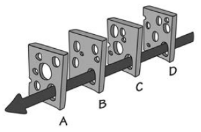
\includegraphics[scale=1]{swisscheesmodel.png}
\end{multicols}
\pagebreak
\subsection{I 5 Perché}
\begin{multicols}{2}
\paragraph{Origine} In origine sono stati sviluppati da Sakichi Toyoda, usati dalla Toyota per milgiorare la qualità dei propri prodotti.
\paragraph{Oggi} Oggi sono ampiamente usati. In pratica, significa che quando si cerca una ragione non bisogna fermarci quando se ne trova una. \textbf{Bisogna chiederci perché}.\\
Poi bisogna chiedercelo di nuovo. Continuare a chiedere finché non si trova la vera causa alla base. Non sono necessariamente 5, ma chiamare questa procedura "I 5 Perché" enfatizza la necessità di continuare a chiedere il perchè anche dopo che una causa è stata trovata.\\\\

\columnbreak
\textbf{Problema}: "Il veicolo non si accende"\\
\textbf{Perché 1} $\longrightarrow$ La batteria è morta\\
\textbf{Perché 2} $\longrightarrow$ L'alternatore non funziona\\
\textbf{Perché 3} $\longrightarrow$ La cinghia dell'alternatore è rotta\\
\textbf{Perché 4} $\longrightarrow$ La cinghia dell'alternatore era ben oltre il suo tempo di servizio e non è stata sostituita\\
\textbf{Perché 5} $\longrightarrow$ Il veicono non è stato mantenuto secondo le tempistiche raccomandate\\
\end{multicols}
\texttt{powernoodle.com/models-article/5-whys}
\subsection{Attitudine delle persone verso gli errori}
\textbf{Non si possono risolvere i problemi a meno che le persone non riconoscano la loro esistenza}. Se si dà la colpa alle persone diventa \textbf{difficile convincere le organizzazioni} a ristrutturare la progettazione per eliminare questi problemi.
\paragraph{Perché le persone commettono errori?} Perché i design si focalizzano sui requisiti del sistema e delle macchine e \textbf{non sui requisiti delle persone}. La maggiorparte dei macchinari richiedono comandi e controlli molto precisi, forzando le persone a inserire le informazioni in maniera impeccabile.\\
\textbf{Ma le persone non sono molto precise}. Le persone sono creature creative, costruttrici ed esploratrici. Sono particolarmente brave a trovare novità, nuovi modi di fare le cose, e vedere nuove opportunità.\\
Requisiti noiosi, ripetitivi e precisi vanno contro questi tratti.
\subsection{Errore}
\textbf{L'errore umano è definito come qualsiasi deviazione dal comportamento "appropriato"}.\\
La parola "appropriato" è tra virgolette perché \textbf{in molte circostanze il comportamento "appropriato" non è conosciuto} o è determinato solo dopo il fatto. Comunque, l'errore è definito come una deviazione dal comportamento generalmente accettato o appropriato.\\
\textbf{Errore è il termine generico per tutte le azioni sbagliate}.
\subsubsection{Lapsus e Errori cognitivi}
Ci sono due classi principali d'errore
\begin{list}{}{}
\item \textbf{Lapsus} (slips)\\
Un \textbf{lapsus avviene quando una persona che intende fare un'azione finisce per farne un'altra}. Con un lapsus, l'azione svolta non è quella che si aveva intenzione di svolgere.
\begin{list}{}{}
\item \textbf{Lapsus di azione} (action based): viene compiuta l'azione sbagliata\\
Esempio: ho versato il latte nella tazza e poi ho messo la tazza in frigo. Azione corretta applicata all'oggetto sbagliato.
\item \textbf{Lapsus di memoria} (memory lapse): la memoria fallisce, quindi l'azione che si intendeva compiere non è compiuta o i suoi risultati non sono valutati.\\
Esempio: mi sono dimenticato di spegnere il gas dopo aver preparato cena.
\end{list}
\pagebreak
\item \textbf{Errori congitivi} (mistakes)\\
Un \textbf{errore cognitivo avviene quando viene stabilito il goal sbagliato} o viene ideato il piano sbagliato. Da quel punto in poi, \textbf{anche le azioni corrette fanno parte dell'errore}, perché le azioni in sé non sono appropriate e fanno parte del piano sbagliato.\\
Con un errore cognitivo, le azioni che vengono compiute rispecchiano il piano: \textbf{è il piano ad essere sbagliato}.
\begin{list}{}{}
\item \textbf{Rule based} mistakes: la persona ha diagnosticato correttamente la situazione, ma ha ideato un piano d'azione sbagliato. Viene seguita la \textbf{regola sbagliata}.\\
Esempio: un meccanico diagnostica un difetto sulla batteria della macchina ma decide di non sostituirla perché funziona ancora al 50\% della capacità.
\item \textbf{Knowledge based} mistakes: la persona ha diagnosticato male il problema a causa di \textbf{conoscenza sbagliata o mancante}\\
Esempio: il peso del carburante viene calcolato in pound invece di chilogrammi.
\item \textbf{Memory lapse} mistakes: avvengono quando vi è una \textbf{dimenticanza} durante le fasi di \textbf{goal, plan o evaluation}.\\
Esempio: un meccanico si distrae e non porta a termine la diagnostica.
\end{list}
\end{list}
\textbf{Slips}: specify/perform, interpret/perceive\\
\textbf{Mistakes}: plan, compare\\
\textbf{I nuovi utenti} sono più portati a compiere \textbf{errori cognitivi} piuttosto che lapsus.\\
\textbf{Gli utenti esperti} compiono più \textbf{lapsus}.\\
Gli \textbf{errori cognitivi} spesso \textbf{nascono da informazioni ambigue o poco chiare} riguardo lo stato corrente del sistema, la \textbf{mancanza di un buon modello concettuale} e procedure inappropriate.
\subsubsection{Prevenzione dell'errore}
\textbf{Non dovrebbe essere possibile, per un semplice errore, causare danno elevato}. Ecco cosa si dovrebbe fare:
\begin{list}{}{}
\item \textbf{Capire} le cause dell'errore e progettare in modo da minimizzare tali cause
\item \textbf{Fare controlli di sensibilità}. Le azioni superano il test del "buon senso"?
\item \textbf{Rendere possibile annullare tali azioni} -- \textit{undo} -- o rendere più difficile fare ciò che non può essere annullato (es. "\textit{Sei sicuro di\ldots?}", lock).
\item \textbf{Rendere più semplice la scoperta di errori da parte delle persone} e rendere più facile la loro correzione.
\item \textbf{Non trattare l'azione come errore}, piuttosto aiuta l'utente a compiere correttamente l'azione. Pensa all'azione come un'approssimazione di ciò che si desidera fare.
\end{list}
\subsection{Interruzioni}
\textbf{L'interruzione è una delle più grandi cause d'errore, specialmente di errori memory-lapse}.\\
Quando un'attività è interrotta da qualche altro evento, il \textbf{costo dell'interruzione è molto maggiore della perdita di tempo richiesta per avere a che fare con l'interruzione}.\\
Per riprendere, è necessario \textbf{ricordare precisamente il precedente stato dell'attività}: qual'era l'obiettivo, a che punto del ciclo d'azione ero e lo stato rilevante del sistema.\\
La maggior parte dei sistemi rende difficile la ripresa a seguito di un'interruzione.
\pagebreak
\section{Alberto Betella, Moonshots and Disruptive Innovation}
\begin{scriptsize}
Alberto Betella, PhD e CTO, Health Moonshot @ Alpha\\\\
\end{scriptsize}
googlex, moonshot: studi per innovazioni future a lungo termine. Telefonica studio per moonshot di salute, rivoluzionare la salute.\\
alhpa.company costruito per i mooneshot.\\
terapie cognitive, esercizi dati alla persona giusta momento giusto posto giusto e usano sensori per estrarre info implicite nell'utente: es segni di pre-depressione, se esco tutti i weekend (rilevo da gps, celle telefoniche) ma poi smetto e non chiamo nessuno può essere segnale d'allarme.
\section{Fabio Viola, Gamification}
Game Designer
\subsection{Gamification}
Il modo di esprimermi in casa visto da poche persone, se spendo pochi euro per esprimermi in un gioco online lo vedono decine di migliaia di persona $\rightarrow$ status sociale.\\
Oggi \textbf{dover fare} viene meno rispetto al \textbf{voler fare}.\\
I software sono ormai quasi sempre personalizzati in qualche modo: prodotti suggeriti, post in bacheca\ldots Non più produzione seriale (prodotti tutti identici, variazione viene eliminata) e utilità per azienda ma \textbf{utilità per l'utente} (Human Centered Design)\\
\textbf{Engagement Centered Design}: progetto per le persone ma anche per \textbf{conquistare il loro \textit{tempo}}, \textit{il tempo è denaro}. \textbf{Sistemi partecipativi}, story-doing contrapposto allo story-telling. Persona parte fondamentale e attiva in grado di modificare e alterare l'esperienza (dosi di coinvolgimento elevate, senso di protagonismo). "\textbf{Io} ho salvato la principessa" contrapposto a "\textbf{Arthur} ha sparato a spoiler". 1a persona vs 3a persona. Prodotto migliore se si adatta alle volontà dell'utente.\\\\
Progettare per le singole persone, nuove gen premiate per la singola partecipazione e non per il paizzamento (gen precedenti premiazione piazzamtno primi 3). Molto più valore sulla collaborazione invece che competizione.\\
Dato microsoft 2013: media d'attenzione è 8s.\\
Libro: Small Data\\
\textbf{Desiderio di completare} muove grossa fette di utenti. è un driver, tra gli altri: pressione sociale, paura di perdere\ldots\\
Storydoing: pubblico modella attivamente narrativa con decisioni anche a modificare il finale. Videogiochi: regno delle decisioni. Non funzionano senza persona che costantemente prende decisioni. Scelte significative sono quelle in cui persone sono: consapevoli, permanenti, con conseguenze e da fare ricordare.\\
\textbf{sony robottino cane famiglia giapponese}\\
creatività, coinvolgimento, collettivi (non si lavora più da soli), contaminazione (inutile 8 ingegneri, ma collettivi misti)\\
\textit{dimmi io dimentico, mostrami io ricordo, coinvolgimi io imparo.} -- Benjamin Franklin\\\\
Libro: Bowling Alone, di Putnam.
\section{Vincenzo Gervasi, Sottosistema Grafico}
Dopo aver progettato interfaccia bisogna implementarla. Tra disp in e disp out (GUI) c'è la nostra interfaccia, da implementare.\\
Insieme alla nostra app c'è un sottostitema grafico che può essere primitiva del S.O.\\
Kernel e sottostitema grafico insieme $\rightarrow$ winzozz\\
Applicazione e sottostitema grafico insieme (S.O. non ha parte grafica) $\rightarrow$ unix <3\\\\
sottosist grafico fornisce serie di operazi da fare tra in e outp in forma digeribile per le applicazioni.
\subsection{sottosistema grafico}
Vari gruppi di operazioni
\begin{list}{}{}
\item da qualche parte si prendono gli input: interfaccia esterna del sttosistema grafico che prende info da disp input\\
Kernel -- Driver I/O implementati sul kernel -- dispositivi input -- sottosistema grafico
\item sottosistema grafico offre interfaccia a applicazioni\\
\textbf{oppure il contrario} applicazione offre interfaccia al sottosist. grafico (inversion of control) il sistema chiama l'app quando ha qualcosa da mostrare (push, appl aspettano che sistema chiami loro interfaccia)
\item Sottosistema grafico ha tante applicazioni da gestire (\textbf{multiplexing}).\\
Multiplexing in tempo dei disp input\\
Multiplexing in spazio bidimensionale del dispositivo di output\\
\item Segnale da input processato e finisce ad un componente  chiamato \textbf{event manager}.
\item Event manager compatta informazioni relative al singolo evento in una struttura dati generata
\item struttura dati evento inserita in coda eventi e ho finito di processare l'evento\\
tutto questo è successo sul thread del S.O. che ha gestito l'interruzione del driver I/O
\item \textbf{event loop} componente che periodicamente estrae eventi dalla coda degli eventi e lo gestisce\\
la coda è importante perché crea disaccoppiamento temporale (momento in cui inserisco diverso dal momento in cui estraggo) quindi thread/processo che inserisce è separato da chi estrae. Coda importante anche perché consente in maniera pulita di gestire concorrenza perché si creano condizioni di racing solo all'accesso alla coda, ma sono facilmente gestibili.
\end{list}
\subsection{modelli}
a finestre, splitscreen, le tab dei browser, alt-tab (multiplexing schermo tra applicazioni schermo intero \textbf{nel tempo})
\subsection{event loop}
\begin{verbatim}
while (!done) {
    msg = cde.get(); //estraggo dalla coda degli eventi facendo i controlli sulla concorrenza
    switch (msg) {
        case KeyDown: if (isQualifier(msg.keyCode)) keyFlags |= flag(msg.keyCode)
                      else if (isValue(...)) ...
                      ...
                      break;
        case MouseMove ...
        ...
    }		
\end{verbatim}
processing immediato, differito (mi segno dati imposto timer quando arriva agisco) o ignorati\\
21/10/2019\\
\textbf{X Server} server che gira sul client che offre delle interfacce grafiche tramite il X11 protocol (protocollo di rete) per cui host (server) su cui girano applicazioni chiama funzioni dell'X server sul client che visualliza \textit{cosa} sullo schermo.\\
X server fornisce istruzioni "accendi pixel a coordinate xy" quindi librerie da usare per astrarre.\\
librerie : java(awt, swing, gdt), obj-c, c++ ne hanno n. Qt, Cocoa su linux. W3c dom\\\\\
\textbf{programmazione ad eventi} paradigma di programmazione distinto da a oggetti, imperativa, funzionale, logica, dichiarativa. Senza multithreading, ognuno degli event loop è un thread, non mi preoccupo di deadlock, race, fairness ecc\ldots perché tutto cade nell'accesso lettura/scrittura nella coda eventi\\
hw -- so -- app (chrome) -- tab -- dom -- javascript -- element (button, img, link\ldots) -- event handler (onClick = "\ldots")\\\\
Dalla grafica si scopre che coda a messaggi e gestione asincrona funziona bene in altri contesti (Es. I/O asincrono in Java NIO)\\\\
\section{Antonio Cisternino, Realizzazione di una GUI}
grafica retantion o immediata\\
windows forms e windows presentation foundation libreria grafiche windows\\
contesto grafico: tavolozza con operazioni grafiche fattibili sui pixel della finestra.\\
finestra solitamente è ciò che trascini chiudi ecc., nel sistema grafico la finestra è un rettangolo di pixel. un bottone tecnicamente è una finestra (vive di vita propria e riceve eventi dal sistema grafico). Le finestre si possono organizzare in alberi.\\
pixel = 1/96 di pollice\\
\textbf{frame buffer}: area di memoria che mappa ogni pixel dello schermo su zona di memoria (solitamente 4Byte, 1 per canale di colore rosso verde blu e 1 byte per il canale alpha cioè trasparenza). 2 gigabyte al secondo per trasmissione 60fps su 4k. Flickering: applicazione scrive nel frame buffer mentre viene letto senza sincronizzazione (scheda video legge quel che c'è e manda non aspetta che il sistema abbia finito il disegno) -- \textbf{double buffering} per risolverla, scrivo già "i pixel giusti" senza aver disegna rettangolo, disenga ellissi ecc in sequenza. contesto grafico non dal frame buffer ma da altra fonte (immagine, stampante\ldots)
\section{Nicola Melluso, Natural Language User Interfaces}
building and deploying a natural language user interface\\
convresational sistem: interfaccia uomo machcina che avviene tramite una conversazione (testuale o vocale). Conversazione interessante perché è naturale: naturalmente conversiamo e scambiamo input così. Perché non usarlo anche per comunicare con il proprio servizio. Inoltre è accessibile: molte volte difficile capire quale tasto premere o i task da fare, se devo semplicemente dirlo l'utente non fa fatica a capire come funziona l'interfaccia.\\
Difficoltà sta nelle sfide per il programmatore: il linguaggio è ambiguo, n modi diversi per dire la stessa cosa. Processo complicato perché pieno di difficotlà.\\
\subsection{Speech recognition e natural language understanding}
AmazonLex definisce "intento" l'obiettivo dell'azione che la macchina deve performare. Riconoscere informazioni chiave all'interno della frase. DataType: gli slot, informazione che nella conversazione è fornita.\\
Intento: obiettivo della nostra conversazione.\\
Utterances: frasi pronunciate\\
Slots: dati necessari per formare l'azione\\
Prompts: risposta che si dà ad ogni azione\\
Fulfillment: \\\\
Lex Bot structure: prima definisco le frasi (utterances), poi gli slot presenti in quelle frasi.
\end{document}